\documentclass[12pt,a4paper]{article}
\usepackage{ctex}
\usepackage{amsmath,amscd,amsbsy,amssymb,latexsym,url,bm,amsthm}
\usepackage{epsfig,graphicx,subfigure}
\usepackage{enumitem,balance}
\usepackage{wrapfig}
\usepackage{mathrsfs,euscript}
\usepackage[usenames]{xcolor}
\usepackage{hyperref}
\usepackage[vlined,ruled,linesnumbered]{algorithm2e}
\usepackage{float}
\usepackage{multirow}
\usepackage{caption}
\hypersetup{colorlinks=true,linkcolor=blue}

\newtheorem{theorem}{Theorem}
\newtheorem{lemma}[theorem]{Lemma}
\newtheorem{proposition}[theorem]{Proposition}
\newtheorem{corollary}[theorem]{Corollary}
\newtheorem{exercise}{Exercise}
\newtheorem*{solution}{Solution}
\newtheorem{definition}{Definition}
\theoremstyle{definition}



\renewcommand{\thefootnote}{\fnsymbol{footnote}}

\newcommand{\postscript}[2]
 {\setlength{\epsfxsize}{#2\hsize}
  \centerline{\epsfbox{#1}}}

\renewcommand{\baselinestretch}{1.0}

\setlength{\oddsidemargin}{-0.365in}
\setlength{\evensidemargin}{-0.365in}
\setlength{\topmargin}{-0.3in}
\setlength{\headheight}{0in}
\setlength{\headsep}{0in}
\setlength{\textheight}{10.1in}
\setlength{\textwidth}{7in}
\makeatletter \renewenvironment{proof}[1][Proof] {\par\pushQED{\qed}\normalfont\topsep6\p@\@plus6\p@\relax\trivlist\item[\hskip\labelsep\bfseries#1\@addpunct{.}]\ignorespaces}{\popQED\endtrivlist\@endpefalse} \makeatother
\makeatletter
\renewenvironment{solution}[1][Solution] {\par\pushQED{\qed}\normalfont\topsep6\p@\@plus6\p@\relax\trivlist\item[\hskip\labelsep\bfseries#1\@addpunct{.}]\ignorespaces}{\popQED\endtrivlist\@endpefalse} \makeatother

\begin{document}
\noindent
\captionsetup[figure]{labelfont={bf},labelformat={default},labelsep=period,name={Fig.}}
%========================================================================
\noindent\framebox[\linewidth]{\shortstack[c]{
\Large{\textbf{Lab10-Turing Machine}}\vspace{1mm}\\
Algorithm and Complexity (CS214), Xiaofeng Gao, Spring 2020.}}
\begin{center}
\footnotesize{\color{red}$*$ If there is any problem, please contact TA Yiming Liu. }

\footnotesize{\color{blue}$*$ Name:Haotian Xue  \quad Student ID:518021910506 \quad Email: xavihart@sjtu.edu.cn}

\end{center}

\begin{enumerate}

\item
Design a one-tape TM $M$ that computes the function $f(x, y) = x \mod y$, where $x$ and $y$ are positive integers ($x > y$). The alphabet is $\{1, 0, \Box, \triangleright, \triangleleft\}$, and the inputs are $x$ 1's, $\Box$ and $y$ 1's. Below is the initial configuration for input $x=7$ and $y=3$. The result $z=f(x, y)$ should also be represented in the form of $z$ 1's on the tape with the pattern of $\triangleright 111 \cdots 111 \triangleleft$.
\begin{center}
	\begin{tabular}{ll|c|c|c|c|c|c|c|c|c|c|c|c|c|c}
		& \multicolumn{14}{c}{Initial Configuration}\\[5pt]
		\cline{2-16}
		& & $\triangleright$ &  1  & 1 & 1 & 1 & 1 & 1 & 1 & $\Box$ & 1 & 1 & 1 & $ \triangleleft$ & \\
		\cline{2-16}
		\multicolumn{2}{c}{} & \multicolumn{1}{c}{$\uparrow$} & \multicolumn{11}{c}{}\\
		\multicolumn{2}{c}{} & \multicolumn{1}{c}{$q_S$} & \multicolumn{11}{c}{}	
	\end{tabular}
\end{center}

\begin{enumerate}
	\item
	Please describe your design and then write the specifications of $M$ in the form like $\langle q_S, \triangleright \rangle \rightarrow \langle q_1, \triangleright,  R\rangle$. Explain the transition functions in detail.
	
	\item
	Please draw the state transition diagram.
	
	\item
	Show briefly and clearly the whole process from initial to final configurations for input $x = 7$ and $y = 3$. You may start like this:
	$$(q_s,\underline{\triangleright}  1  1  1  1  1  1  1  \Box 1  1  1   \triangleleft)
	\vdash (q_1,\triangleright  \underline{1}  1  1  1  1  1  1  \Box 1  1  1   \triangleleft)
	\vdash^* (q_1,\triangleright  1  1  1  1  1  1  1  \underline{\Box} 1  1  1   \triangleleft)
	\vdash (q_2,\triangleright  1  1  1  1  1  1  1  \Box \underline{1}  1  1   \triangleleft)$$
	
	\par{\color{blue}(Note that for simplicity, we write $(q_1,\triangleright  \underline{1}  1  1  1  1  1  1  \Box 1  1  1   \triangleleft)\vdash^* (q_1,\triangleright  1  1  1  1  1  1  1  \underline{\Box} 1  1  1   \triangleleft)$ if the corresponding transaction repeats on multiple inputs with the same state.)}
	
\end{enumerate}



\begin{solution}
The solutions for this problem is as following.

(a) I implement the mod operation  $x~mod ~y$by repeatedly substract $y$ from $x$ untill x is not big enough to be substracted.
And the Turing Machine process can be divided into three parts: the main substract loop and two conditional jumps.
That is, in the main loop, we repeat the substract of $x$ by turning some $1s$ in the end of $x$ into $0s$.
The first conditional jump is for the bits in $y$, when $y$ become all-zeros, we turn it into all-ones to make the next substraction. The other jump happens when $x$ is turned into all-zeros
but $y$ is not, which means we should turn  some $0s$ of $x$ into $1s$, and we call it resume operation.

We have many states in the implementation and they are:


\begin{itemize}
	\item \textbf{$q_1$}: this is also the starting state, in this state we move right to the end of $y$.
	\item \textbf{$q_2$}: in this state we turn the last $1$ of $y$ into $0$.
	\item \textbf{$q_3$} :move to the end of $x$.
	\item \textbf{$q_4$} : change the last $1$ in $x$ into $0$.
	\item \textbf{$q_5$}: move to the starting point and repeat substraction.
	\item \textbf{$q_6$}: when $y$ become all-zeros, make $y$ all-ones.
	\item \textbf{$q_7$}: when $x$ is all-zeros, move the end of $y$.
	\item \textbf{$q_8$}: move to the last $0$ in $y$.
	\item \textbf{$q_9$}: move to the last $1$ in $x$.
	\item \textbf{$q_{10}$}: resume operation.
	\item \textbf{$q_{11}$}: $y$ is all-zeros and resume operation is done.
	\item \textbf{$q_{12}$}: move to the end of $x$.
	\item \textbf{$q_{H}$}: turn the fisrt $0$ in $x$ into the end notation.
\end{itemize}

Main substraction loop:($q_1 \sim q_5$), jump1($q_6$), jump2($q_7 \sim q_{12} +  q_H$).

$M$ is designed as follows, and to make it more briefly to read, $\langle q, (a_1, a_2, ..., a_i) \rangle \rightarrow \langle q, (b_1, b_2, ..., b_i)),  R\rangle$ means:
$\langle q, a_k \rangle \rightarrow \langle q, b_k,  R\rangle(k = 1, 2, ..., i)$.

$\langle q_1, (0,1,\Box,\triangleleft) \rangle \rightarrow \langle q_1, (0,1,\Box,\triangleleft),  R\rangle$ 

 $\langle q_1, \triangleleft \rangle \rightarrow \langle q_2, \triangleleft,  L\rangle$ // move to the end of $y$

$\langle q_2, 1 \rangle \rightarrow \langle q_3, 0,  L\rangle$ // change the last $1$ in $y$ into $0$

$\langle q_3, 1 \rangle \rightarrow \langle q_3, 1,  L\rangle$

$\langle q_3, \Box \rangle \rightarrow \langle q_4, \Box,   L\rangle$ 

$\langle q_4, 1 \rangle \rightarrow \langle q_5, 0,   L\rangle$ // turn the last $1$ of $x$ into $0$ 

$\langle q_5, \triangleright \rangle \rightarrow \langle q_5, /triangleright,   R\rangle$ // return to starting point

$\langle q_2, \Box \rangle \rightarrow \langle q_6, \Box,   R\rangle$ // jump then $y$ is all $0s$

$\langle q_6, 1 \rangle \rightarrow \langle q_6, 0,   R\rangle$ // make $y$ into all $1s$

$\langle q_6, \triangleleft \rangle \rightarrow \langle q_2, \triangleleft,   L\rangle$ $y$ is all make into $1$ 

$\langle q_4, \triangleright \rangle \rightarrow \langle q_7, \triangleright,   R\rangle$ // begin to resume

$\langle q_7, (1, 0, \Box) \rangle \rightarrow \langle q_7, (1, 0, \Box),   L\rangle$ 

$\langle q_7, \triangleleft \rangle \rightarrow \langle q_8, \triangleleft,   L\rangle$ 

$\langle q_8, 1 \rangle \rightarrow \langle q_8, 1,   L\rangle$ // turn to the last $0$ in $y$

$\langle q_8, 0 \rangle \rightarrow \langle q_9, 1,   L\rangle$ // change the last $0$ of $y$ into $1$

$\langle q_9, (0, \Box) \rangle \rightarrow \langle q_9, (0, \Box),   L\rangle$

$\langle q_9, (0, \triangleright) \rangle \rightarrow \langle q_{10}, (0, \triangleright),   L\rangle$ // move to the first $0$ in $x$

$\langle q_{10}, 0 \rangle \rightarrow \langle q_7, 1,   R\rangle$ //write the first $0$ in $x$ into $1$ and repeat the resume operation

$\langle q_8, \Box \rangle \rightarrow \langle q_{11}, \Box,   L\rangle$

$\langle q_{11}, 0 \rangle \rightarrow \langle q_{11}, 0,   L\rangle$  // find the first $0$ in $x$

$\langle q_{11}, 1 \rangle \rightarrow \langle q_{12}, 1,   L\rangle$ 

$\langle q_{12}, 0 \rangle \rightarrow \langle q_{H}, \triangleleft,   L\rangle$ 



(b) State transition diagram is shown is Fig 1.


\begin{figure}
	\centering
	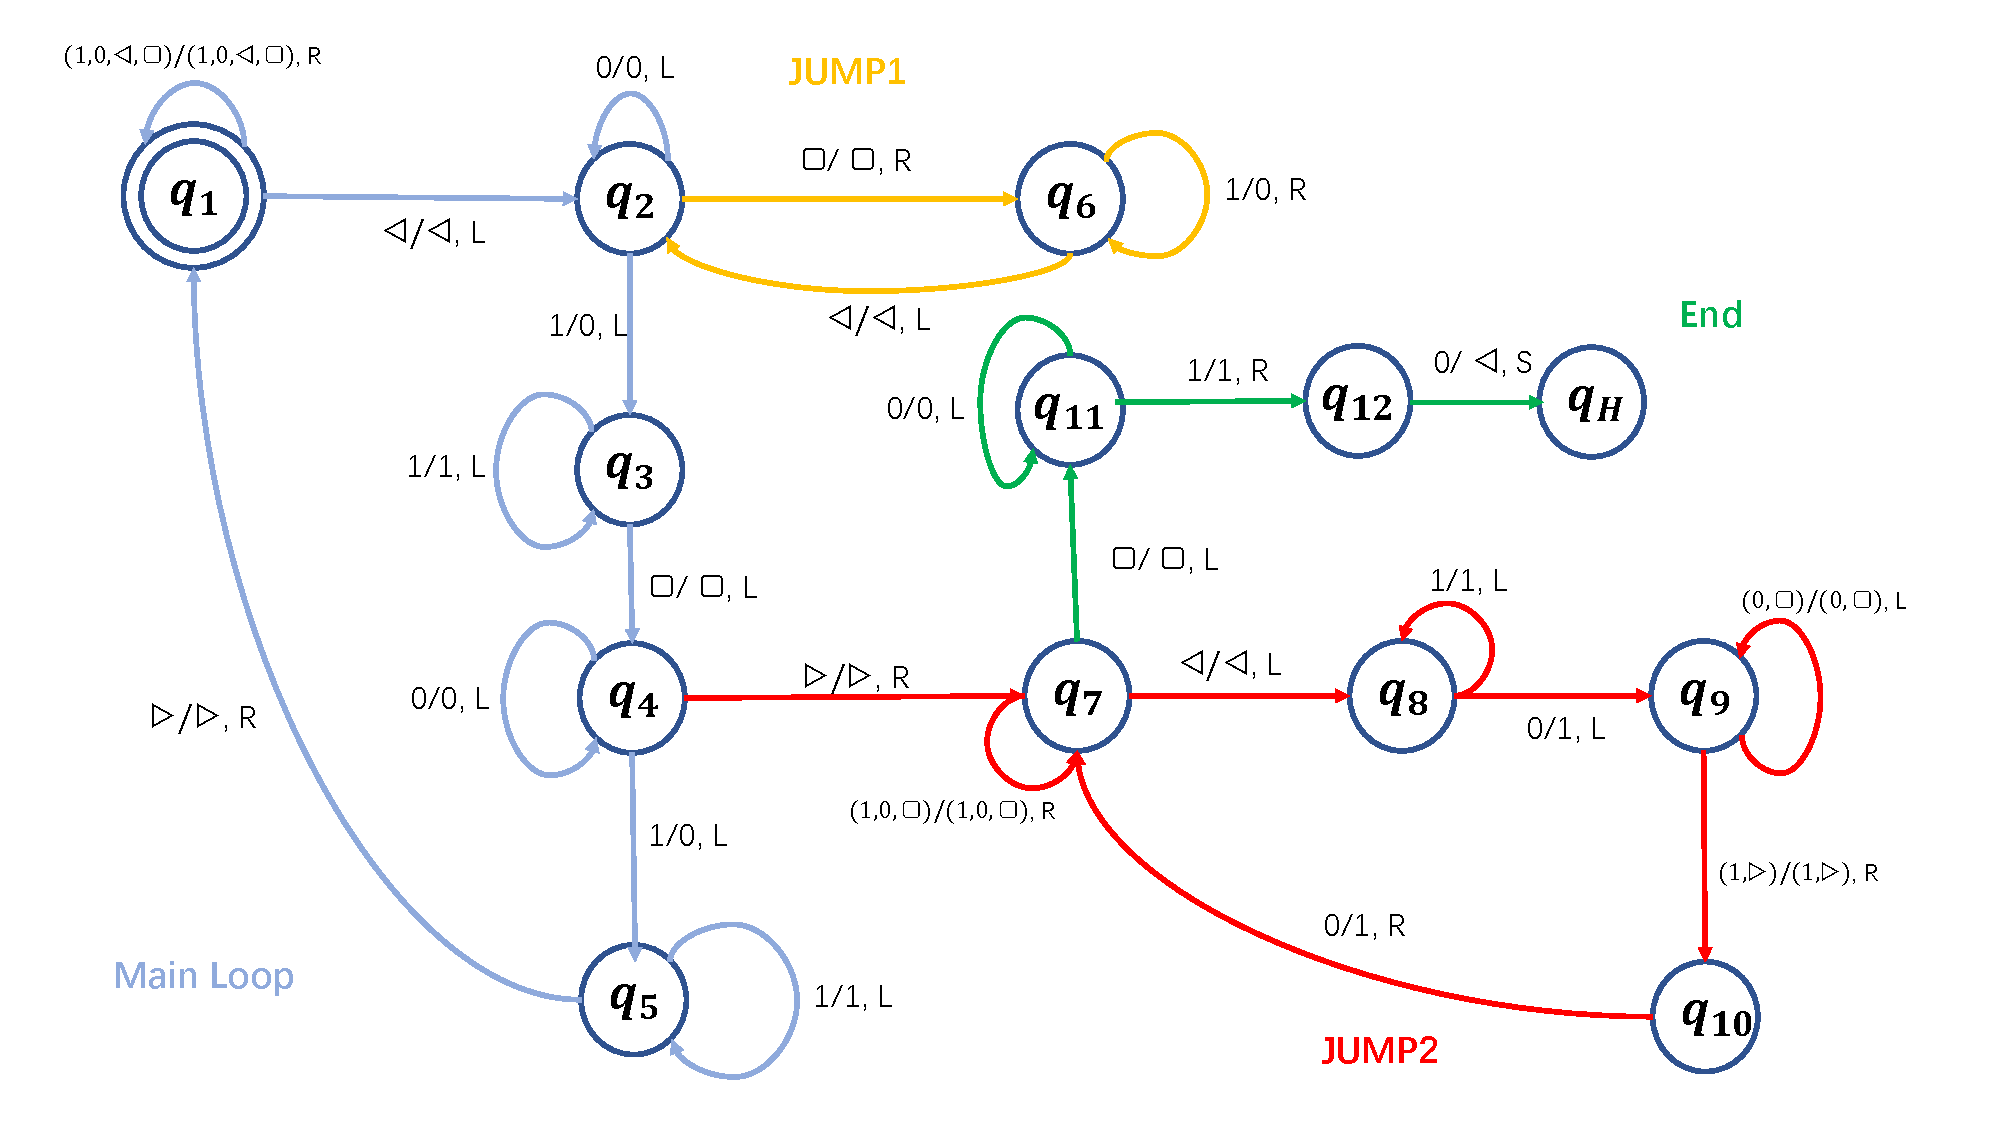
\includegraphics[scale=0.5]{TM.pdf}
    \caption{Problem 1-(b)}

\end{figure}



(c) To make the answer of this part more briefly to read, I will divided the process into two main sections and in each
section there are some subsections, and I will ommit some of the subsections since they are the same to work.

\begin{itemize}
	\item \textbf{Substract $3$ from $7$}($7 - 3 = 4$)  
	$\vdash (q_1,\underline{\triangleright}  1 1  1  1  1  1  1  \Box 1  1  1   \triangleleft)$

	$\vdash^{*} (q_1,\triangleright  1  1  1  1  1  1  1  \Box 1  1  \underline{1}   \triangleleft)$

	$\vdash (q_2,\triangleright  1  1  1  1  1  1  1  \Box 1  1  \underline{1}  \triangleleft)$

	$\vdash (q_3,\triangleright  1  1  1  1  1  1  1  \Box 1  1  \underline{0}  \triangleleft)$

	$\vdash (q_4,\triangleright  1  1  1  1  1  1  \underline{1}  \Box 1  1  0  \triangleleft)$
	
	$\vdash (q_5,\triangleright  1  1  1  1  1  1  \underline{0} \Box 1  1  0   \triangleleft)$

	$\vdash^{*} (q_5,\triangleright  \underline{1}  1  1  1  1  1 0 \Box 1  1  0   \triangleleft)$

	$\vdash (q_1,\underline{\triangleright}  1 1  1  1  1  1  0  \Box 1  1  0  \triangleleft)$

	we ommit the other two $sub-1$ operations and directly turn to the conditional jump:
	
	$\vdash (q_1,\underline{\triangleright}  1 1  1  1  0 0  0  \Box 0 0  0  \triangleleft)$

	$\vdash^{*} (q_1,\triangleright  1  1  1  1  0 0 0  \Box 0  0  \underline{0}   \triangleleft)$

	$\vdash (q_2,\triangleright  1  1  1  1  0  0  0  \underline{\Box}  0 0 0  \triangleleft)$

	$\vdash (q_6,\triangleright  1  1  1  1  0  0  0  \Box  \underline{1} 0 0  \triangleleft)$

	$\vdash^{*} (q_6,\triangleright  1  1  1  1  0  0  0  \Box  1 1 \underline{1}   \triangleleft)$

	$\vdash (q_2,\triangleright  1  1  1  1  0  0  0  \underline{\Box}  1 1 1 \triangleleft)$

 
	
	So we successfully turn $3$ into $111$ and we continue the substraction untill $7$ becomes $0000000$:
   
	\item \textbf{Resume operation:}
	
   $\vdash (q_1,\underline{\triangleright}  0 0 0 0  0 0  0  \Box 1 1  0  \triangleleft)$

   $\vdash^{*} (q_1,\triangleright  0 0 0 0 0 0 0  \Box 1 1 0   \triangleleft)$

   $\vdash (q_2,\triangleright  0 0 0 0  0 0 0  \underline{\Box} 1  1  0   \triangleleft)$

   $\vdash (q_3,\triangleright  0 0 0 0  0 0 0  \underline{\Box} 1  1  0   \triangleleft)$

   $\vdash (q_4,\triangleright  0 0 0 0  0 0  \underline{0}  \Box 1  1  0   \triangleleft)$

   $\vdash^{*} (q_4,\underline{\triangleright}  0 0 0 0  0 0 0  \underline{\Box} 1  1  0   \triangleleft)$

   $\vdash (q_7,\triangleright  0 0 0 0  0 0 0  \Box 1  1  0  \underline{\triangleleft)}$

   $\vdash (q_8,\triangleright  0 0 0 0  0 0 0 \Box 1  1 \underline{0}   \triangleleft)$

   $\vdash^{*} (q_8,\triangleright  \underline{0} 0 0 0  0 0 0 \Box 1  1  1 \triangleleft)$

   $\vdash (q_9,\triangleright  \underline{0} 0 0 0  0 0 0 \Box 1  1  1 \triangleleft)$

   $\vdash (q_{10},\triangleright  \underline{1} 0 0 0  0 0 0 \Box 1  1  1 \triangleleft)$

   $\vdash (q_{7},\triangleright  \underline{1} 0 0 0  0 0 0 \Box 1  1  1 \triangleleft)$


   And then we turn to check if $3$ is all ones and end the process:

   $\vdash^{*} (q_{7},\triangleright  1 0 0 0  0 0 0 \Box 1  1  1 \underline{\triangleleft})$

   $\vdash (q_{8},\triangleright  1 0 0 0  0 0 0 \underline{\Box} 1  1  1 \triangleleft)$
  
   $\vdash (q_{11},\triangleright  1 0 0 0  0 0 \underline{0} \Box 1  1  1 \triangleleft)$

   $\vdash^{*} (q_{11},\triangleright  \underline{1} 0 0 0  0 0 0 \Box 1  1  1 \triangleleft)$

   $\vdash (q_{12},\triangleright  1 \underline{0}  0 0  0 0 0 \Box 1  1  1 \triangleleft)$

   $\vdash (q_{H},\triangleright  1 \underline{\triangleleft}  0 0  0 0 0 \Box 1  1  1 \triangleleft)$


   












\end{itemize}

\end{solution}





\item Assume there's a Turing Machine $M$ using alphabet $\Gamma :\{ \triangleright, \Box, a, b, \cdots, z\}$. We can simulate $M$ by a Turing Machine $\tilde{M}$ using alphabet $\tilde{\Gamma }:\{ \triangleright, \Box, 0, 1\}$. Please transform the instruction $\langle q, i \rangle \rightarrow \langle q',j, R\rangle$ in $M$ into its corresponding form in $\tilde{M}$.


\item \textbf{Wireless Data Broadcast System.}
In a Wireless Data Broadcast System (WDBS), data items are repeatedly broadcasted in cycle on different channels. Denote $D = \{d_1, d_2,\cdots, d_k\}$ as data items, each $d_i$ with length $l_i$ (as time units), and $\mathbf{C}=\{C_1, C_2, \cdots, C_n\}$ as broadcasting channels. Fig. illustrates a WDBS with 25 data items and 4 channels. Once a channel finishes broadcasting current cycle, it will repeat these data again as a new cycle. E.g., a possible broadcasting sequence of $C_1$ could be \{$d_6$, $d_{12}$, $d_1$, $d_{18}$, $d_7$, $d_6$, $d_{12}$, $d_1$, $d_{18}$, $d_7$, $\cdots$\}

\begin{figure}[h]
	\centering
	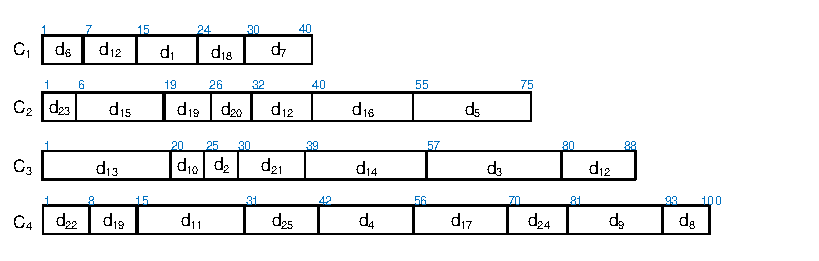
\includegraphics[scale=1]{Fig-Broadcast.pdf}
	\caption{An Example Scenario of Wireless Data Broadcast System.} \label{Fig-Broadcast}
\end{figure}

If a mobile client requires a subset of data items $D_q \subseteq D$ from this WDBS, he/she must access onto one channel, wait for the appearance of one required item, and switch to another channel if necessary. Each ``switch'' requires one time slot. For example, Lucien wants to download $\{d_1, d_3, d_5\}$, as shown in Fig.. He firstly accesses onto $C_1$ at time slot 1, then download $d_1$, $d_3$ respectively during time slots 2 to 5, and then switch to $C_3$ at time slot 6 (note that he cannot download $d_5$ from $C_2$ because of the switch constraint), and download $d_5$ during time slots 7 to 8. We define \emph{access latency} as the period when a client starts downloading, till the time he/she finishes. As a result, the overall access latency for Lucien is 7 in this example.

\begin{figure}[!htbp]
	\centering
	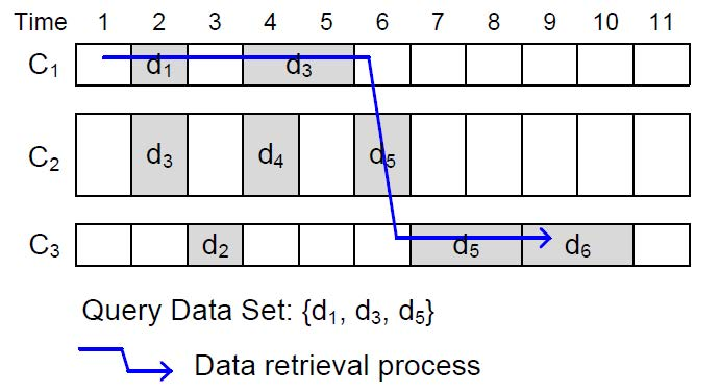
\includegraphics[scale= 0.5]{Fig-Access.pdf}
	\caption{An Example Scenario of Query of a Client.} \label{Fig-Access}
\end{figure}

Each operation (download/wait/switch) needs energy consumption. To conserve energy, a client hopes to use minimum amount of energy to download all required items in $D_q$, which means that he/she waits to minimize both access latency and switch numbers. Unfortunately, these two objectives conflict with each other naturally. Fig. exhibits such a scenario. To download $D_q=\{d_1, d_2, d_3, d_4\}$, if we start from $C_2$, in Option 1 we can switch to $C_1$ for $d_1$ immediately after downloading $d_3$, return back to $C_2$ for $d_4$, and to $C_1$ again for $d_2$. Such option costs 3 switches and 7 access latency. While in Option 2, we stay at $C_2$ lazily for $d_3$ and $d_4$, and then switch to $C_1$ for $d_2$ and $d_1$. Such option costs 1 switches and 12 access latency.


\begin{figure}[!htbp]
	\centering
	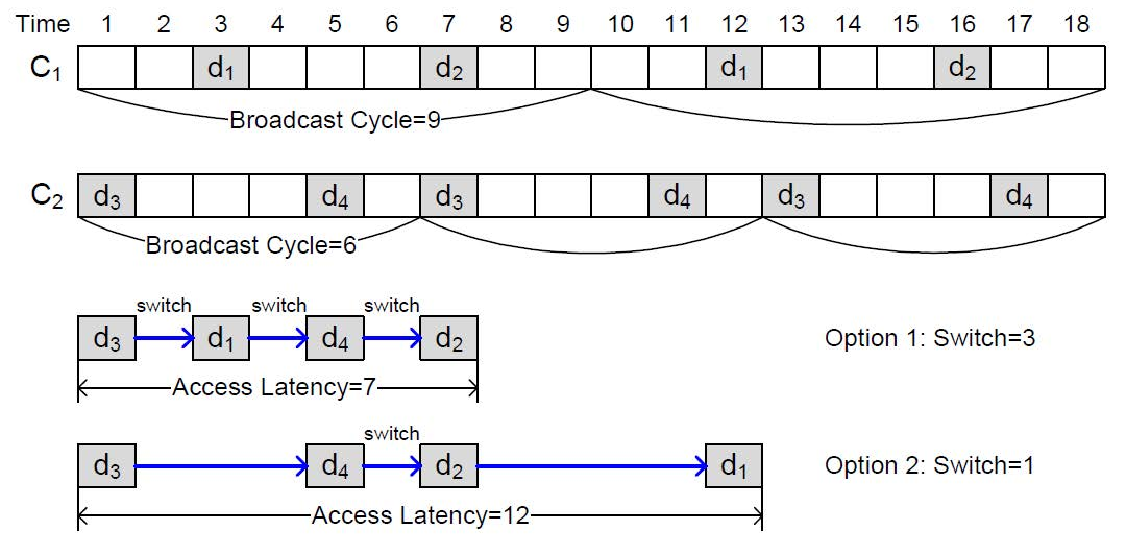
\includegraphics[scale= 0.5]{Fig-Conflict.pdf}
	\caption{Confliction between Access Latency and Switch Number.} \label{Fig-Conflict}
\end{figure}

Once we want to minimize two conflictive objectives simultaneously, we have three possible ways (similar as Segmented Least Squares told in Dynamic Programming Lecture). Now it is your turn to complete the formulation of this optimization, we name it as Minimum Constraint Data Retrieval Problem (MCDR), with the following sub-questions.
\begin{enumerate}
	\item If we add an additional switch parameter $h$, please define the MCDR (Version 1) completely as a search problem.
	\item If we add an additional latency parameter $t$, please define the MCDR (Version 2) completely as a search problem.
	\item If we set dimensional parameters $\alpha$ to switch number, and $\beta$ to access latency, we can combine two objectives together linearly as a new concept ``cost''. Please define the Minimum Cost Data Retrieval Problem (MCDR, Version 3) correspondingly.
	\item Please give the decision versions of sub-questions (a), (b) and (c).
\end{enumerate}
\end{enumerate}

%========================================================================
\end{document}
